	\paragraph{}
	En este capítulo expondremos el trabajo que se pretende realizar para conseguir cada uno de los objetivos mostrados en el capítulo anterior.
	
\section{Objetivo principal del proyecto}

	\paragraph{}
	Se desarrollará una aplicación gráfica multiplataforma, mediante la herramienta \emph{Unity3D} utilizando el motor gráfico que incluye, para alojar el simulador de tráfico.
	
	\paragraph{}
	Debido a problemas con Unity3D en la generación de la aplicación para sistemas Linux y a la imposibilidad de realizar pruebas sobre el sistema operativo de Apple, la aplicación será finalmente construida para el sistema operativo Windows en sus versiones de 32 y 64 bits.

\section{Red viaria}

	\paragraph{}
	La red viaria que utilizará el simulador vendrá especificada en un fichero con formato GraphML \cite{GraphML_man}. Dicha red estará determinada por dos grafos, un grafo no dirigido, de topología, en el que los cruces, las curvas y los nodos límite (los puntos de entrada/salida de vehículos desde y hacia la porción de red viaria simulada) serán los nodos, y las vías serán los arcos; y un grafo dirigido, para indicar los giros, en el que los carrilles de las vías serán los nodos y los giros serán los arcos.
	
	\paragraph{}	
	Debido a las restricciones que impone la definición de GraphML sobre los identificadores, cada grafo deberá estar en un fichero distinto. Para ello usaremos dos ficheros por cada red viaria, siendo los ficheros *.topology.graphml para el primer tipo de grafo y los ficheros *.turns.graphml para el segundo. El identificador del grafo en cada uno de los ficheros de la pareja de cada grafo será el mismo.
	
	\paragraph{Nodos del grafo de topología}
	
	\paragraph{}
	Debemos distinguir tres tipos:
	\begin{itemize}
		\item \underline{Nodos de cruce}: Representan un cruce de vías típico. El grado de estos nodos es tres o cuatro.
		
		\begin{figure}[H]
			\centering
				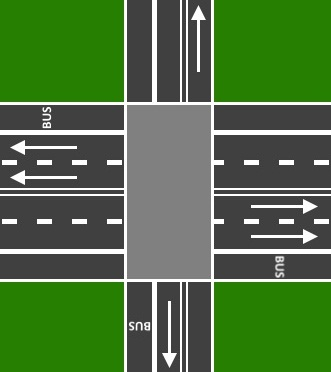
\includegraphics[keepaspectratio,height=100px]{Nodo_cruce.jpg}
		\end{figure}
	
		\item \underline{Nodos de límite de vía}: Representan el límite del área simulada en esa vía. Será el lugar por el que los vehículos salgan y entren desde y hacia la porción de red viaria simulada. El grado de este tipo de nodo es igual a uno. En el entorno 3D tendrán apariencia de tunel.
		
		\begin{figure}[H]
			\centering
				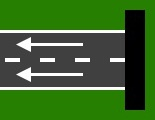
\includegraphics[keepaspectratio,height=50px]{Nodo_limite.jpg}
		\end{figure}
	
		\item \underline{Nodos de continuación}: Representan ángulos en las vías de tal forma que en ellos no se producirán intersecciones de vías. El grado de este tipo de nodo es igual a dos.
		
		\begin{figure}[H]
			\centering
				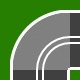
\includegraphics[keepaspectratio,height=50px]{Nodo_continuacion.jpg}
		\end{figure}
	
	\end{itemize}
	
	\paragraph{}
	Por tanto, cada nodo estará definido por un identificador alfanumérico, el tipo de nodo (0: nodo de cruce, 1: nodo de límite de vía, 2: nodo de continuación), sus coordenadas en el plano bidimensional x,y, y para los nodos de tipo cruce, el tipo de cruce, cruce normal (0) o rotonda (1). Las rotondas se han quedado como punto de ampliación de la aplicación.
	
	\paragraph{Arcos del grafo de topología}	
	\paragraph{}
	Cada arco estará definido por un identificador alfanumérico, el nodo de origen, el nodo de destino, una cadena de texto para poder dar nombre a la vía, y dos cadenas de texto que servirán para indicar los tipos de carril en cada sentido.
	
	\paragraph{}
	Cada una de las cadenas de tipo de carril especificará el tipo de carril o carriles de ese sentido que haya desde el exterior de la vía hacia el interior de la misma utilizando los códigos: P: para indicar un carril de transporte público, N: un carril normal, o la cadena `0' para indicar que no hay carriles en ese sentido.
	
	\paragraph{Nodos del grafo de giros}
	
	\paragraph{}
	Cada nodo estará definido por un identificador alfanumérico que se corresponderá con uno de los identificadores de los carriles de los arcos del grafo de topología. Los identificadores de los carriles tendrán la forma siguiente: identificador del arco al que pertenece, guión bajo, la cadena ``src\_des" o la cadena ``des\_src" en función de la dirección en la que va el carril, (desde el origen al destino o viceversa), guión bajo, número de carril desde el exterior del arco hacia el interior, siendo 0 el primer carril.
	\paragraph{}
	Por ejemplo, el segundo carril del arco ``a2" en dirección origen destino será:
	\begin{lstlisting}
		<node id="a2_src_des_1"/>
	\end{lstlisting}
	
	\paragraph{Arcos del grafo de giros}
	
	\paragraph{}
	Cada arco estará definido por un identificador alfanumérico, el nodo de origen y el nodo de destino. Si el arco está definido significa que el giro está permitido. En el caso de carriles que lleguen a nodos de tipo continuación o límite, no será necesario definir los arcos.
	
	\paragraph{Ejemplo}
	Para ilustrar esta especificación vamos a ver un ejemplo de red viaria y cuál sería su representación en GraphML.
	
	\begin{figure}[H]
		\centering
			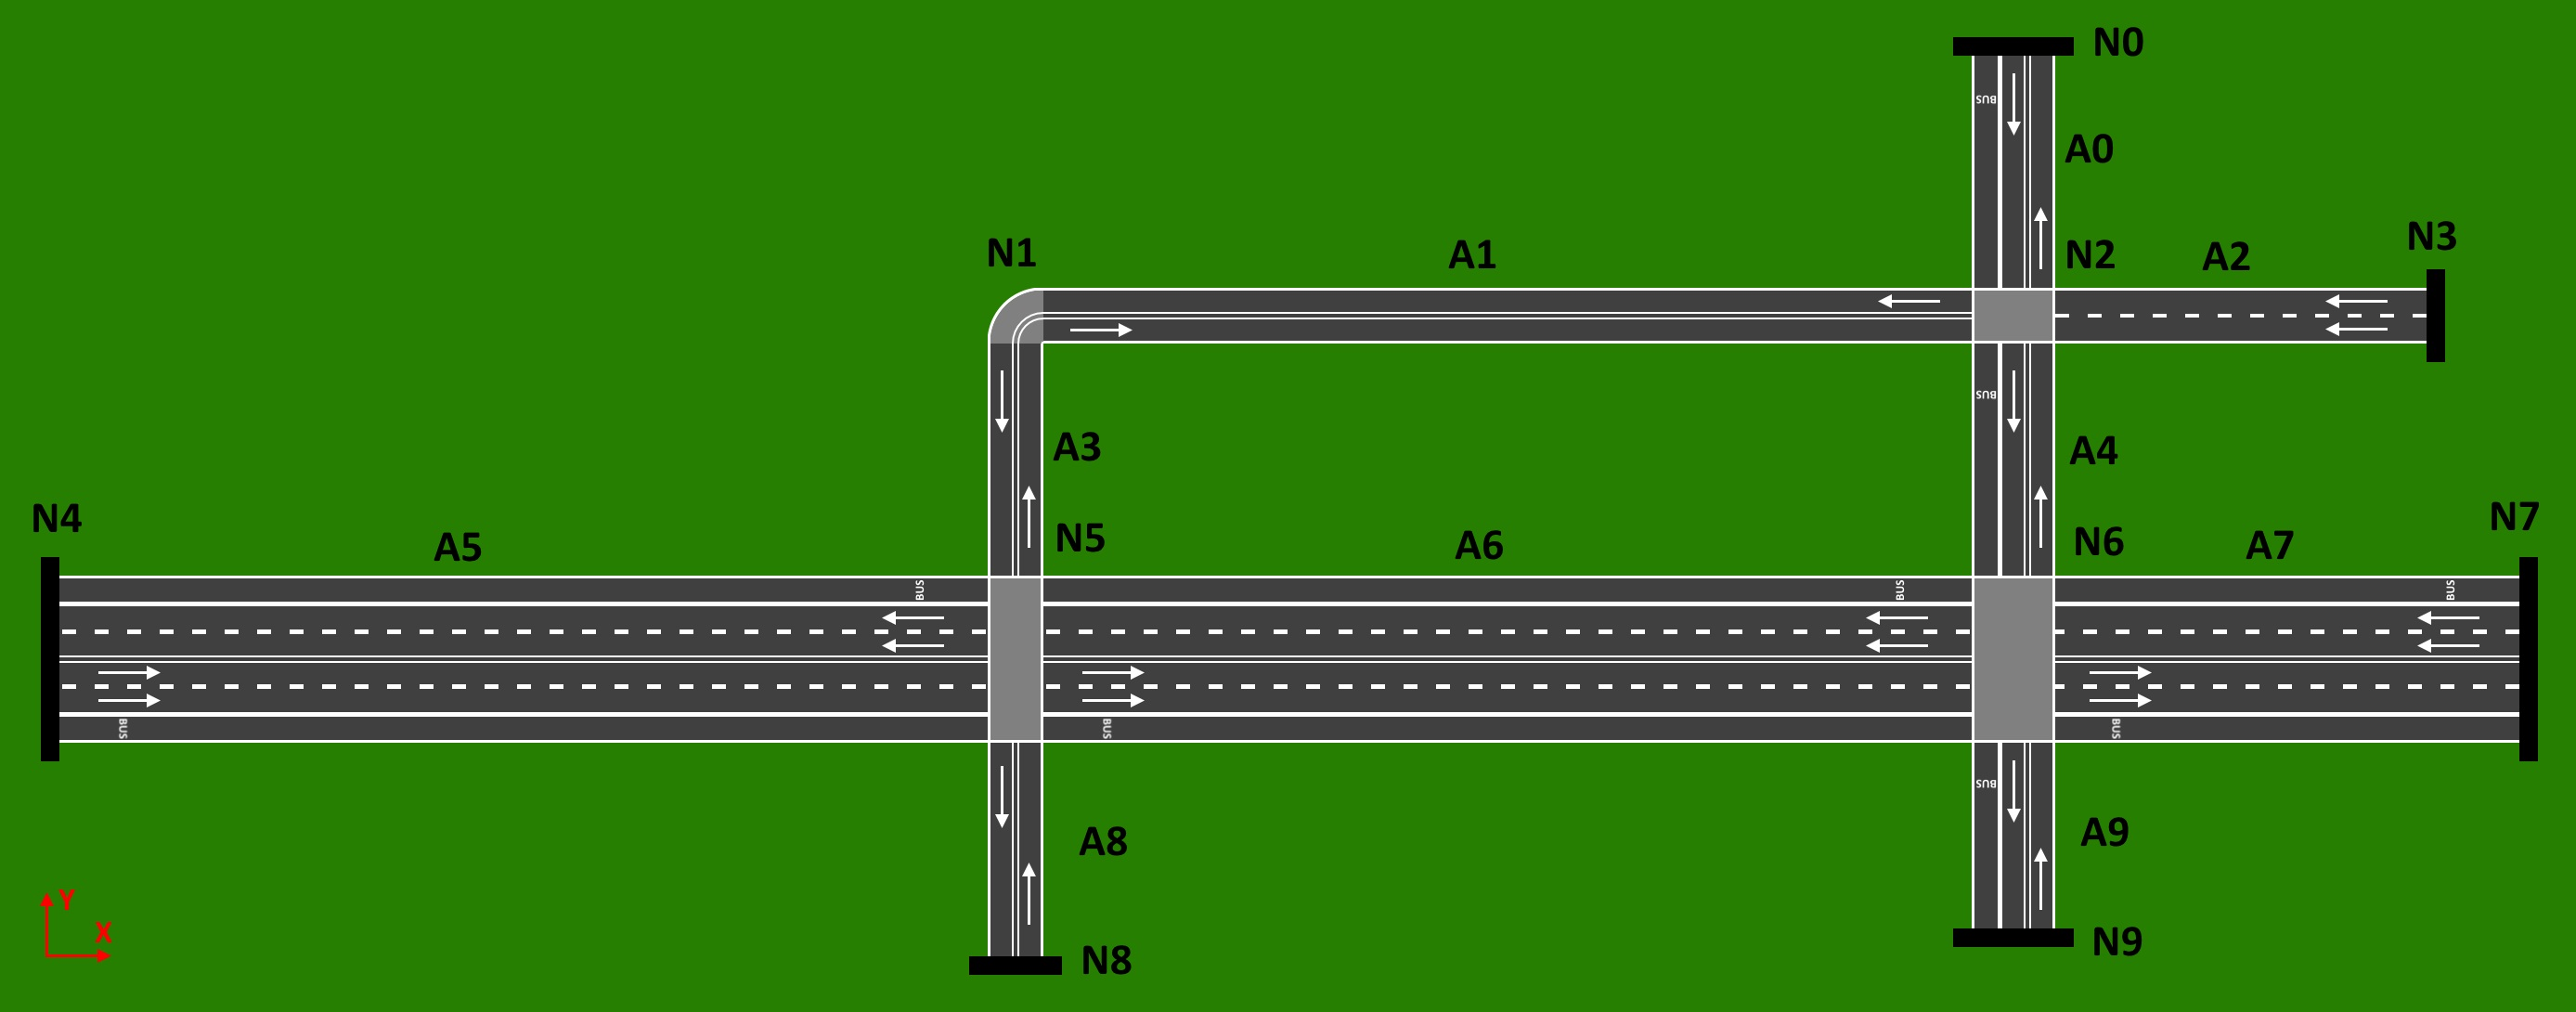
\includegraphics[keepaspectratio,width=359px]{Ejemplo_red_vial.jpg}
	\end{figure}
	
	\paragraph{}
	Como se puede apreciar en la imagen, el grafo de topología asociado consta de diez nodos, tres nodos de tipo cruce, un nodo de tipo continuación y seis nodos de tipo límite de vía. Además, el grafo cuenta con diez arcos que representan las vías de la imagen.
	
	\paragraph{}
	Para este ejemplo se ha supuesto que en cada cruce se puede ir en todas las direcciones que admite esta red, aunque se aprovecha la multiplicidad de carriles para hacer los giros a izquierda desde el carril o carriles situado/s más a la izquierda, y análogamente con los giros a la derecha.
	
	\paragraph{}
	El grafo de giros está compuesto por diez nodos, los arcos del grafo de topología, que en este ejemplo están todos presentes en el grafo debido a que todos están unidos a algún nodo de tipo cruce; y treinta y tres arcos que representan los giros.
	
	\paragraph{}
	A continuación se mostrará la representación de la red viaria con sintaxis de GraphML.
	
	\paragraph{}
	Grafo de topología:
	\tiny
	\lstinputlisting{"../Traffic Flow Simulator/Assets/StreamingAssets/Maps/example_1.topology.graphml"}
	\normalsize
	\paragraph{}	
	Grafo de giros:
	\tiny
	\lstinputlisting{"../Traffic Flow Simulator/Assets/StreamingAssets/Maps/example_1.turns.graphml"}
	\normalsize
	
\section{Señales de tráfico}

	\paragraph{}
	Como se mencionó anteriormente, las señales con las que cuenta el simulador son semáforos de tres estados. Estos semáforos han sido modelados por mi en Blender \cite{Blender_web} e importados en Unity3D.
	
	\begin{figure}[H]
		\centering
			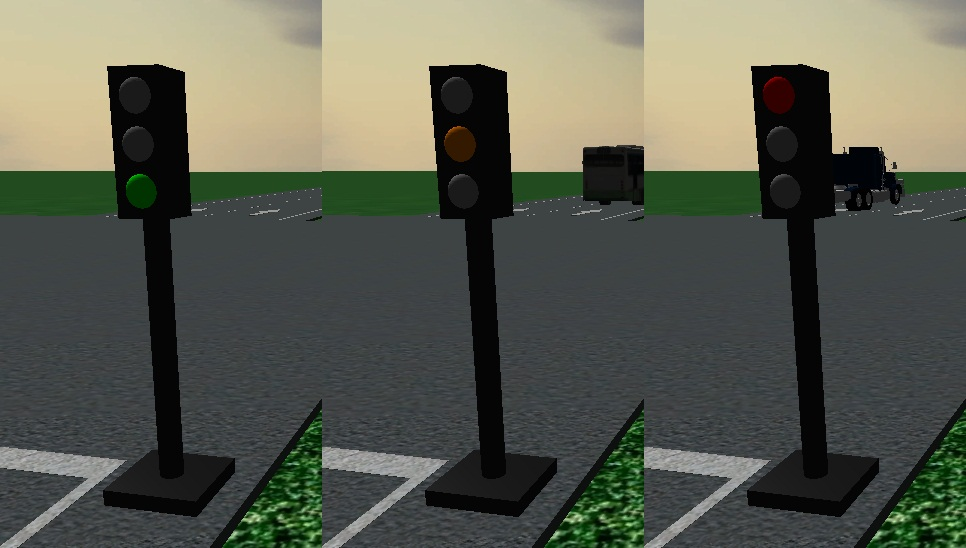
\includegraphics[keepaspectratio,height=150px]{TrafficLightThreeState.jpg}
	\end{figure}
	
	Su funcionamiento consiste en realizar un ciclo contínuo desde el estado rojo, pasando después a verde, luego a naranja y, finalmente, a rojo de nuevo.
	
	\paragraph{}	
	El tiempo que tardan en ponerse en verde por primera vez vendrá determinado por el número de semáforos que haya en un cruce. Se decide aleatoriamente el orden en el que se pondrán en verde y a partir de ahí se calcula el tiempo de retardo para comenzar el ciclo de tal forma que cada semáforo del cruce permanecerá en rojo el tiempo que los demás semáforos utilizan para sus estados verde y naranja.

\section{Vehículos}
	
	\paragraph{}
	Se importarán los siguientes modelos utilizando la herramienta Blender \cite{Blender_web} o el propio importador de modelos obj de Unity3D:
	\begin{itemize}
		\item Bus
		\item Taxi Checker Marathon
		\item Chevrolet Camaro
		\item Todoterreno verde
		\item Todoterreno naranja
		\item Cabeza tractora camión
	\end{itemize}
	
	\paragraph{}	
	Estos modelos no han sido realizados por mi, han sido tomados de lugares con las licencias adecuadas.
	
	\paragraph{}
	Una vez cargados en Unity3D se han ajustado sus escalas en el editor de forma que respetasen en la medida de lo posible las proporciones en las medidas entre unos vehículos y otros.
	
\section{Conductores}

	\paragraph{}
	Para simular la lógica de los conductores se ha utilizado un modelo muy básico fundamentándose en tres tipos de conductor:
	
	\begin{itemize}
	\item Buenos
	\item Regulares
	\item Malos
	\end{itemize}
	
	Los buenos conductores respetan la señalización de los semáforos en todo momento, los conductores regulares la respetan con una probabilidad del 50\%, mientras que los malos conductores no respetarán dicha regulación en ningún momento.
	
\section{Entorno}

	\paragraph{}
	El entorno está formado por un suelo con textura de hierba y un skybox para formar el cielo. Los nodos límite son falsos túneles modelados por mi en Blender \cite{Blender_web} e importados en Unity3D.
	
	